\documentclass[serif,mathserif]{beamer}
%\documentclass[handout]{beamer}
\usepackage{amsmath, amsfonts, epsfig, xspace}
\usepackage{algorithm,algorithmic}
\usepackage{pstricks,pst-node}
\usepackage{multimedia}
\usepackage[normal,tight,center]{subfigure}
\setlength{\subfigcapskip}{-.5em}
%\usepackage{beamerthemesplit}
\usetheme{lankton-keynote}
\usepackage[utf8x]{inputenc}
\usepackage[T1]{fontenc}
\setbeamertemplate{footline}[frame number]

\author[Stefan Sobek]{Stefan Sobek}

\title[Masterarbeit\hspace{2em}\insertframenumber/\inserttotalframenumber]{Implementierung eines Webservices nach \\ ISO 29002-31
Query for characteristic data}

\date{6. März 2014} %leave out for today's date to be insterted

\institute{Fernuni Hagen \\ Fakultät für Mathematik und Informatik \\ Lehrgebiet Datenbanksysteme für neue Anwendungen \\ Betreuer: Dr. Wolfgang Wilkes}

\begin{document}

\maketitle

%\section{Introduction}  % add these to see outline in slides

\begin{frame}
  \frametitle{Überblick}
\begin{columns}
        \column{.45\textwidth}
 \begin{itemize}
  \item Aufgabenbeschreibung
    \begin{itemize}
    \item Problemstellung
    \item Lösungsoptionen
    \item Zielsetzung
    \item Gesamtkontext und Abgrenzung
    \item Lieferketten
    \end{itemize}
  \item Anforderungsanalyse
    \begin{itemize}
    \item Analyse ISO 29002-31
    \item Analyse ISO 22745-30
    \item Use Cases
    \end{itemize}
     \end{itemize}
  
     \column{.55\textwidth}
   \begin{itemize}  
    \item System- und Softwareentwurf
    \begin{itemize}
    \item Auswahlprozess
    \item Architektur
    \end{itemize}
  
   \item Implementierung
    \begin{itemize}
    \item Configuration Management
    \item Webservice
    \item Query Verarbeitung
    \item Transformation
    \item Fehlerbehandlung
    \item SOAP-Webservice
    \end{itemize}    
    \item Schlußfolgerung  
 \end{itemize}
\end{columns}
\end{frame}

\begin{frame}
  \frametitle{Aufgabenbeschreibung - Problemstellung}
  Heutiger automatisierter Produktdatenaustausch zwischen Systemen
  \begin{itemize}
  \item Schnittstellen für Datenaustausch basieren auf definierte Schemata
  \item häufig starres Schema z.B. ein konkretes Werkzeug wäre
      \begin{description}
      \item[ID] 4711
      \item[NAME] Schraubendreher
      \item[LÄNGE] 10cm 
      \item[TYP] Kreuz 
      \end{description}
  \item bieten Methoden an welche Modelldaten liefern ( z.B. getItemNameBy(IRDI) )
  \item dadurch oft unflexibel durch fest verdrahtetes Modell 
  \item Änderungen der Semantik, Struktur oder Inhalte führt zu Modelländerungen und zu hohen Kosten durch Anpassungen beim Klienten
  %leave out the  on the final item
  \end{itemize}
\end{frame}

%\section{Main Body} % add these to see outline in slides

\begin{frame}
  \frametitle{Aufgabenbeschreibung - Lösung}
  Zusätzliche Ebene als Abfrage- und Antwortschnittstelle
  \begin{itemize}
  \item ist flexibel
  \item einheitliche Schnittstelle
  \item dadurch bei Einhaltung keine Änderungen notwendig
  \end{itemize}
  Beispielabfragen
      \begin{description}
      \item[Abfrage 1] Gib mir die Eigenschaften NAME, LÄNGE und den TYP des Elementes mit der ID 4711
      \item[Abfrage 2] Gib mir die Eigenschaft LÄNGE des Elementes mit NAME = 'Schraubendreher'
      \end{description}
\end{frame}

\begin{frame}
  \frametitle{Aufgabenbeschreibung - Lösung}
  Es bieten sich vorhandene ISO-Standards für flexible Abfrage- und Antwortschnittstellen an, z.B.:
  \begin{itemize}
  \item ISO 22745-35 - Open technical dictionaries and their application to master data: Query for characteristic data
  \item ISO 29002-31 - Exchange of characteristic data: Query for characteristic data
  \end{itemize}
  Vorteile
    \begin{itemize}
  \item Definierte Syntax
  \item abgekoppelt vom Domänenmodell
  \item nutzen Ontologien
    \end{itemize}
\end{frame}

\begin{frame}
  \frametitle{Aufgabenbeschreibung - Zielsetzung}
  Implementierung einer flexiblen Abfrage- und Antwortschnittstelle 
  \begin{itemize}
  \item Analyse der ISO 29002-31 - Query for characteristic data
     \begin{itemize}
     \item Betrachtung nach Möglichkeiten einer herkömmlichen SQL-Schnittstelle (Projektion, Selektion)
     \item Definieren von Use Cases
     \end{itemize}
  \item Prototypische Implementierung basierend auf ISO 29002-31 - Query for characteristic data
      \begin{itemize}
      \item Datenbasis PLIB Datenbank
      \item Nutzung vorhandener Prozeduren der PLIB-Datenbank
      \end{itemize}
  \end{itemize}
\end{frame}

\begin{frame}
  \frametitle{Aufgabenbeschreibung - Gesamtkontext und Abgrenzung}
    Abschlussarbeiten um die PLIB
  \begin{figure}[t]
    %\centering
    %\subfigure[First Frame]{
    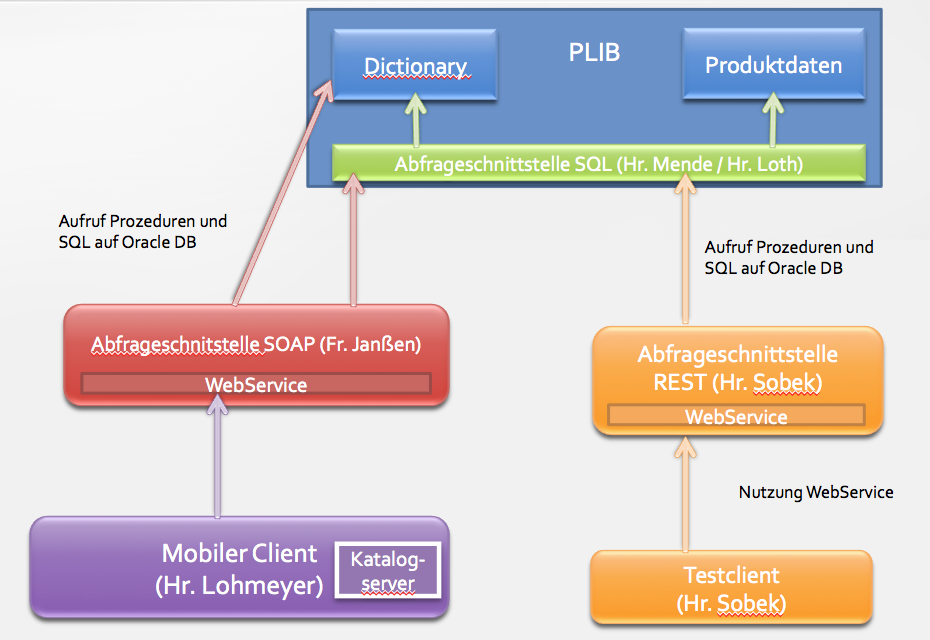
\includegraphics[width=7.5cm]{images/gesamtkontext_plib.png}
    %\subfigure[Middle Frame]{
    %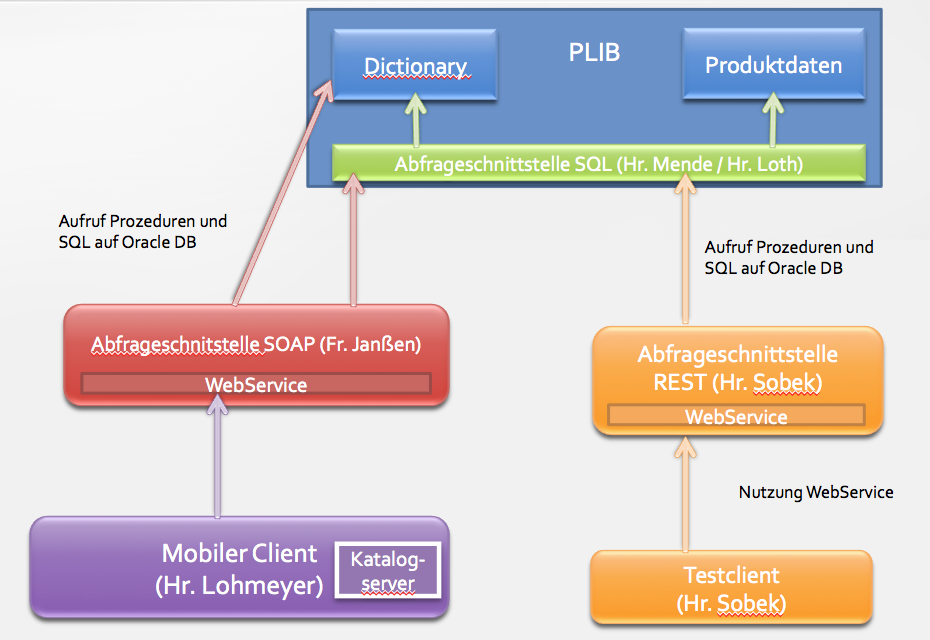
\includegraphics[width=3cm]{images/gesamtkontext_plib.png}}
    %\subfigure[Last Frame]{
    %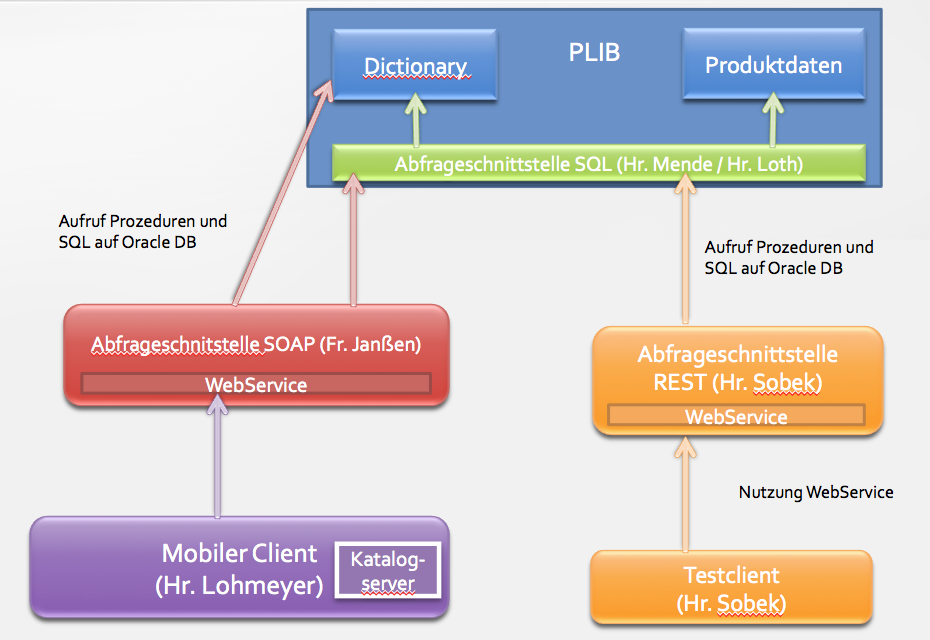
\includegraphics[width=3cm]{images/gesamtkontext_plib.png}}
  \end{figure}
\end{frame}

\begin{frame}
  \frametitle{Aufgabenbeschreibung - Lieferketten}

  \begin{figure}[t]
    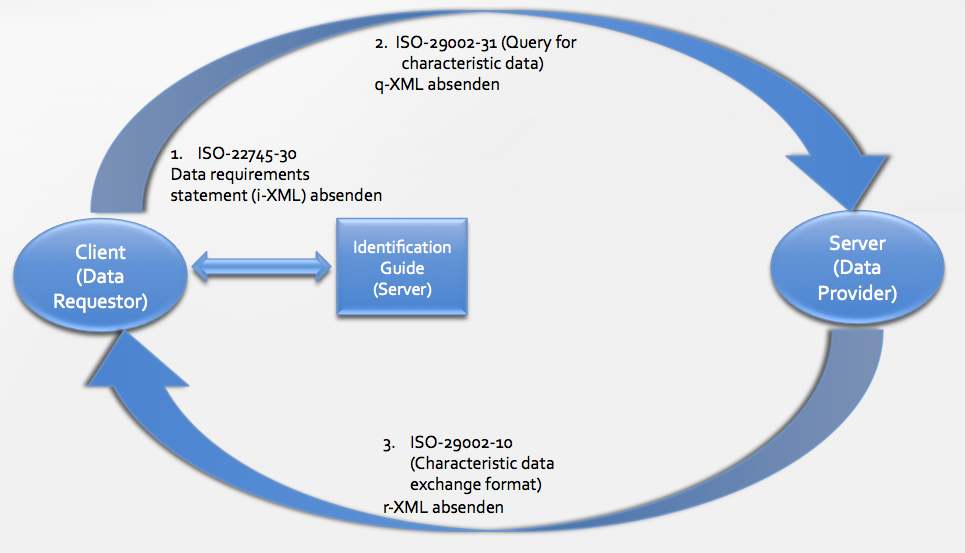
\includegraphics[width=9.5cm]{images/lieferketten_plib.png}
  \end{figure}
\end{frame}

% \section{Conclusion} % add these to see outline in slides

\begin{frame}
  \frametitle{Anforderungsanalyse}
  \begin{itemize}
  \item Analyse ISO 29002-31 - Exchange of characteristic data
    \begin{itemize}
    \item Simple Query (Projektion) \\ z.B. analog SQL: SELECT <attributnamen> FROM TABELLE
    \item Parametric Query (Selektion) \\ z.B. analog SQL: SELECT * FROM TABELLE WHERE <attribut> >= X
    \end{itemize}
  \item Analyse ISO 22745-30 - Identification Guide
    \begin{itemize}
    \item Zusätzliche Einschränkung der Anforderungen an die Daten
    \item Für reine Abfrage analog zu SQL nicht notwendig
    \end{itemize}  
  \end{itemize}
\end{frame}

\begin{frame}
  \frametitle{Anforderungsanalyse}
  Use Cases
    \begin{figure}[t]
    %\centering
    %\subfigure[First Frame]{
    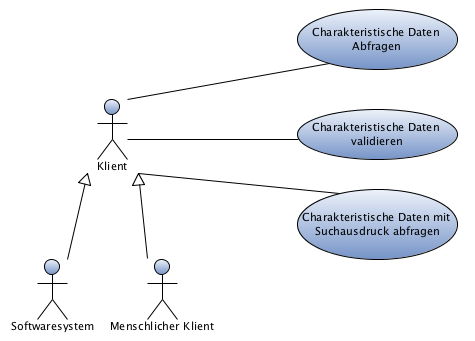
\includegraphics[width=7.5cm]{images/usecases_plib.png}
    %\subfigure[Middle Frame]{
    %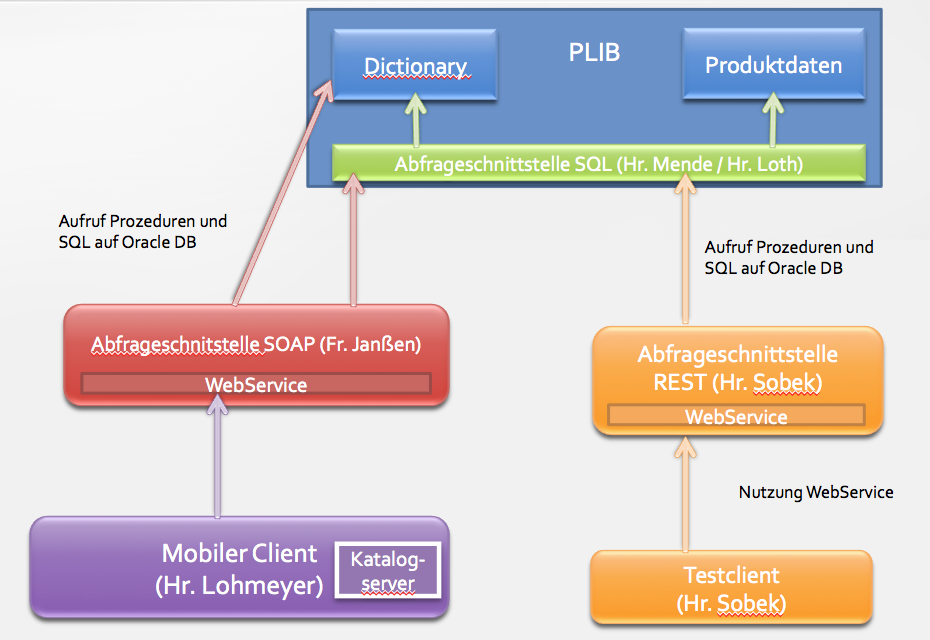
\includegraphics[width=3cm]{images/gesamtkontext_plib.png}}
    %\subfigure[Last Frame]{
    %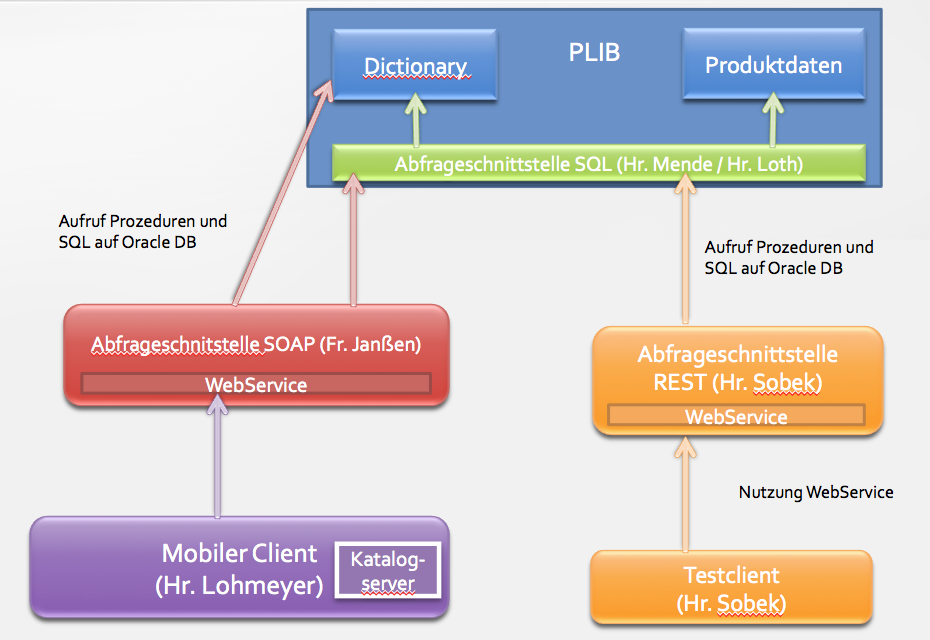
\includegraphics[width=3cm]{images/gesamtkontext_plib.png}}
  \end{figure}
\end{frame}

\begin{frame}
  \frametitle{System- und Softwareentwurf}
  Auswahlprozess
  \begin{itemize}
  \item Webservice
  	  \begin{itemize}
	  \item RESTful Webservice ausgewählt
           \item SOAP bereits in PLIB-Abschlussarbeit Fr. Janßen eingesetzt
           \item in diesem Anwendungsfall kein Vorteil von SOAP gegenüber REST
           \item RESTful Webservice kein Standard sondern Programmierparadigma
           \item basiert auf HTTP-Protokoll
           \end{itemize} 
   \item Java und Apache Tomcat Webserver
  	  \begin{itemize}
           \item weit verbreitet
           \item ermöglicht sowohl SOAP als auch REST
           \end{itemize} 
  \end{itemize}
\end{frame}

\begin{frame}
  \frametitle{System- und Softwareentwurf}
  Softwaredesign und Architektur
  \begin{itemize}
  \item Kontextabgrenzung
     \begin{figure}[t]
     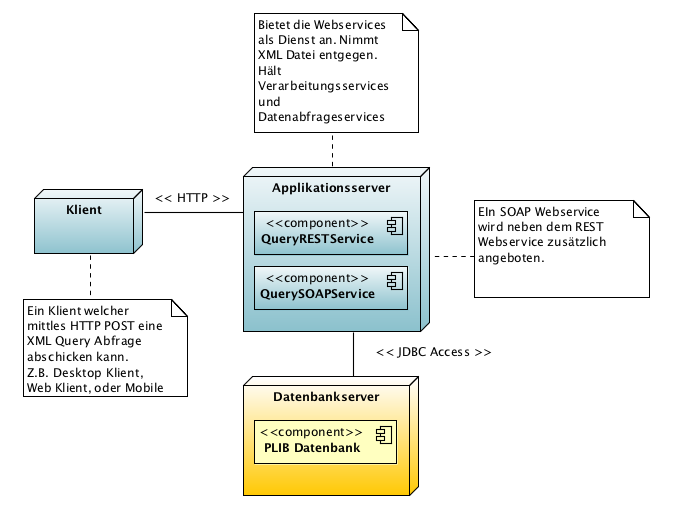
\includegraphics[width=7.5cm]{images/bausteinsicht_plib_level0.png}
     \end{figure}
  \end{itemize}
 \end{frame}
 
 \begin{frame}
  \frametitle{System- und Softwareentwurf}
  Softwaredesign und Architektur
  \begin{itemize}
  \item Bausteinsicht - Level 1 - Whiteboxsicht 
     \begin{figure}[t]
     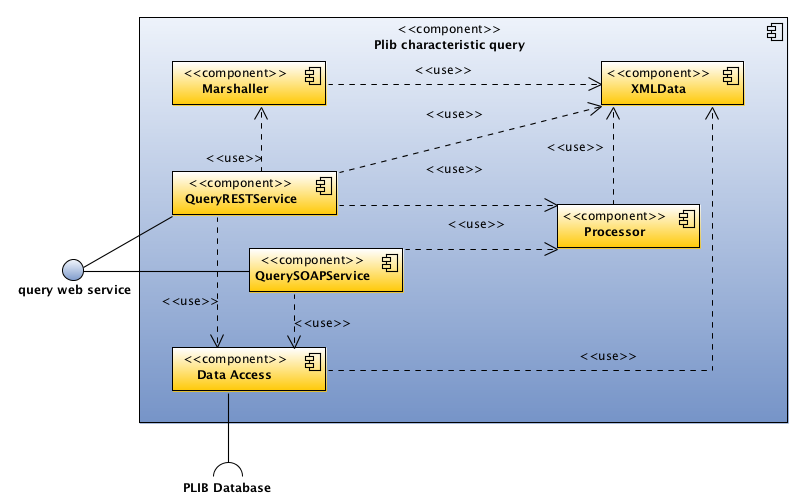
\includegraphics[width=7.5cm]{images/bausteinsicht_plib_level1.png}
     \end{figure}
  \end{itemize}
 \end{frame}

\begin{frame}
  \frametitle{Implementierung}
  Configuration Management
  \begin{itemize}
  \item Versionsverwaltung mit GIT
  \item Build Management mit Maven
  \item Automatische Entwicklertests mit JUnit
  \item Manuelle Entwicklertests mit CURL und GUI-Tester
  \end{itemize}
\end{frame}

\begin{frame}
  \frametitle{Implementierung}
  Notwendige Schritte für Query Verarbeitung (Unmarshalling)
  \begin{enumerate}
  \item Ein Modell in Java erstellen
  \item XML parsen und in Modell überführen
  \item Validierung des Modells anhand der Regeln aus Schema-Datei
  \end{enumerate}
  
  \begin{description}
\item[Modellgenerierung] Mittels Java JAXB aus XSD-Dateien (Schemadateien der ISO 29002-31), in Maven Buildprozess integriert worden
\item[XML parsen] Mittels JAXB Unmarshalling 
\item[Validierung] Mittels JAXB Schemavalidierung
\end{description}

\end{frame}


\begin{frame}
  \frametitle{Implementierung}
 Transformation und Abfrage PLIB Prozeduren
\begin{description}
\item[GET\_PROP\_VALS\_STRING] IN-Parameter ist eine Externe Produkt-ID, liefert eine Tabelle vom Typ PROP\_STRING\_NTT 
Werte: 
  \begin{description}
  \item[IRDI] Eindeutiger Identifier der Teileeigenschaft.
  \item[VALUE] Wert der mittels IRDI identifizierten Teileeigenschaft.
  \item[UNIT] Einheit der Teileeigenschaft.
  \item[PREFIX] Prefix für den konkreten Wert.
  \item[TOLERANCE] Wertetoleranzangabe.
  \item[VALUE\_ID] Identifier des konkreten Wertes.
  \end{description}

  \end{description}
  
  Weitere Prozeduren für andere Datentypen, z.B.: GET\_PROP\_VALS\_NUMBER...
  \end{frame}

\begin{frame}
  \frametitle{Implementierung}
  Sequenzdiagramm eines Simple Queries
    \begin{figure}[t]
    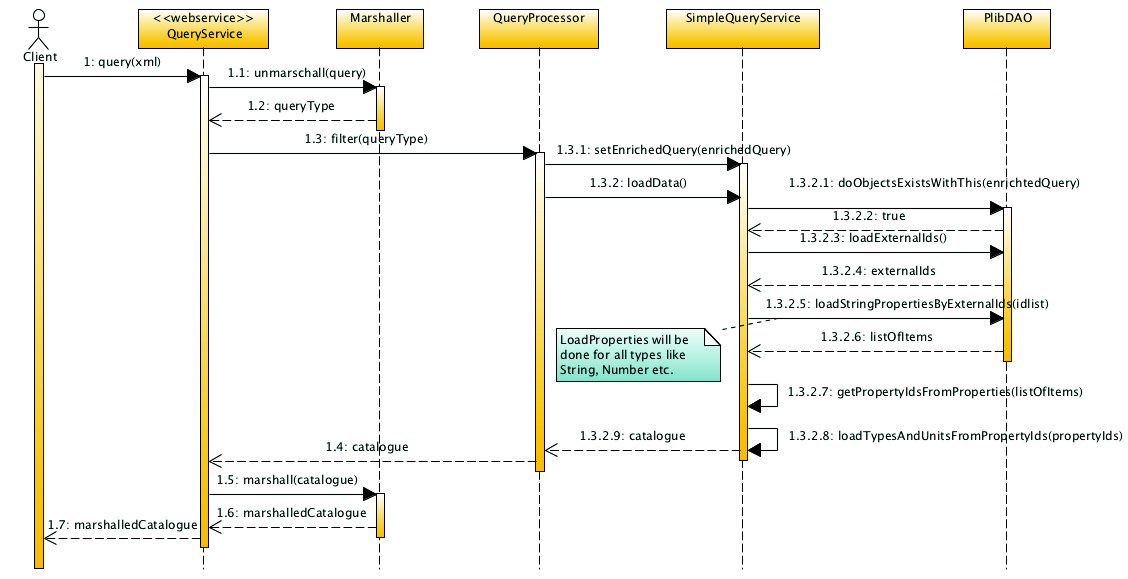
\includegraphics[width=11.5cm]{images/plib_simple_query_sequence_diagram.jpg}

  \end{figure}
\end{frame}


\begin{frame}
  \frametitle{Implementierung}
  Problemstellung - externer Identifier 
  \begin{itemize}
  \item query.xsd bezieht sich auf IRDI, z.B. "Gib mir alle Eigenschaften der Instanzen eines Skalpells mit Identifier 0173-1\#01-BAD803\#2  (IRDI )
  \item Problem: IRDI nicht als IN-Parameter der Prozeduren vorhanden
  \end{itemize}
  
  Mögliche Lösungen
   \begin{enumerate}
  \item Anpassen der Datenbank Prozeduren
  \item Separate Abfrage zur Ermittlung der IRDIs
  \end{enumerate}
  
  \begin{description}
\item[Separate Abfrage wurde als Lösung gewählt, da sehr simpel] SELECT o.DI\_ID FROM DE\_CLASS c, DO\_OBJECT o WHERE c.ID = o.C\_ID AND c.IRDI = ? 
\end{description}

\end{frame}


\begin{frame}
  \frametitle{Implementierung}
  Problemstellung - Aufruf der Oracle Prozeduren mit Java
  \begin{itemize}
  \item GET\_PROP\_VALS\_STRING konnte nicht aufgerufen werden
  \item Rückgabetyp: PACK\_PROPERTY.PROP\_STRING\_NTT wird nicht erkannt
  \item SQLJ Developers Guide: "Oracle SQLJ and JDBC do not support calling arguments or return values of the PL/SQL BOOLEAN type or RECORD types"
  \end{itemize}
  
  Mögliche Lösungen
   \begin{enumerate}
  \item Datenbank ohne Prozeduren abrufen
  \item Anpassen der Datentypen in Oracle, Benutzung von OBJECT-Types anstatt RECORD-Types.
  \end{enumerate}
  
  \begin{description}
\item[Datentypenanpassung] Herr Mende hat freundlicherweise die OBJECT Types erstellt (z.B. PROP\_STRING\_OBJ)
\end{description}

\end{frame}

\begin{frame}
  \frametitle{Implementierung}
 Fehlerbehandlung
  \begin{itemize}
  \item Keine Fehlerbehandlung im Standard definiert
  \item Wie bekommt der Aufrufer z.B. einen Validierungfehler mitgeteilt?
  \end{itemize}
  
 Mögliche Lösungen
   \begin{enumerate}
  \item Bei Fehler immer leeren Katalog zurückgeben 
  \item Fehler-Schema definieren 
  \item Fehlerhandling mittels Protokoll (z.B. HTTP oder SOAP)
  \end{enumerate}
  
  \begin{description}
\item[Fehler Schema definiert] Es wurde ein Fehler-Schema definiert, da Implementierung sonst pro Protokoll nötig. 
\end{description}

  
\end{frame}


 \begin{frame}
  \frametitle{Implementierung}
  Fehlerbehandlung - Error Schema

     \begin{figure}[t]
     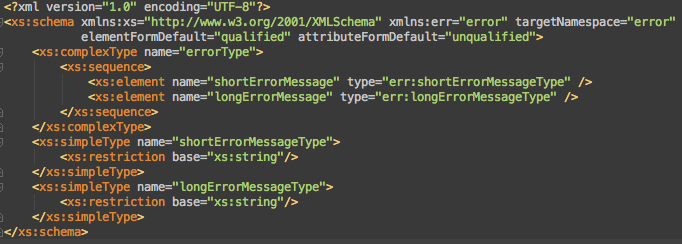
\includegraphics[width=10cm]{images/ErrorSchema.png}
     \end{figure}
 \end{frame}

 \begin{frame}
  \frametitle{Implementierung}
  Fehlerbehandlung - Error Schema in Katalog-Schema eingebunden

     \begin{figure}[t]
     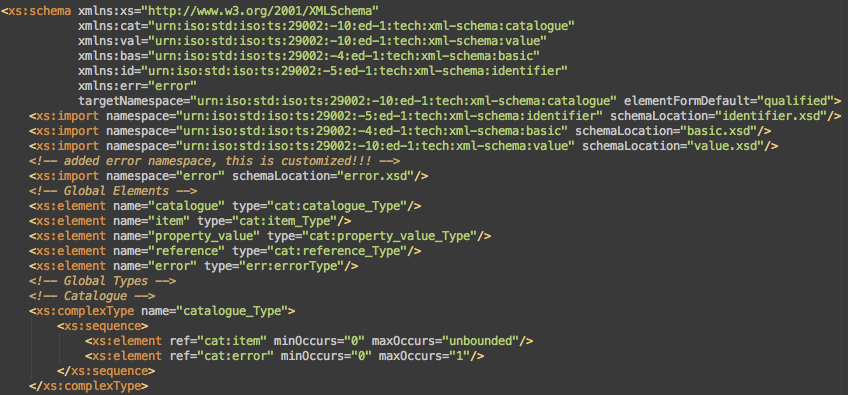
\includegraphics[width=11.5cm]{images/ErrorSchemaCatalogue.png}
     \end{figure}
 \end{frame}

 \begin{frame}
  \frametitle{Implementierung}
  Demonstration
  
     \begin{itemize}
     \item Mittels CURL
          \begin{itemize}
          \item Simple Query (Projektion)
          \end{itemize}
     \item Mittels Test-GUI
          \begin{itemize}
          \item Simple Query (Projektion)
          \item Simple Query - eine Property
          \item Simple Query - Multiple Properties
          \item Simple Query - Validierung (bekanntes Item)
          \item Simple Query - Illegal Query (falsch formatierte IRDI)
          \item Parametric Query - Range (Selektion)
          \item Parametric Query - Range MIN
          \item Parametric Query - Range MAX
          \item Parametric Query - Range with AND
          \end{itemize}   
        \item Abfrage SOAP-Webservice mit SOAP-UI              
     \end{itemize}
 \end{frame}


\begin{frame}
  \frametitle{Schlußfolgerung}
  
  \begin{itemize}
	\item Prototyp von flexibler Schnittstelle gemäß ISO 29002-31 erfolgreich implementiert
	\item PLIB als Datenbasis angebunden und Anfragedaten transformiert
	\item Implementierung als RESTful Webservice
	\item SOAP-Implementierung später einfach möglich, da Modell bereits vorhanden
	\item Test-GUI implementiert 
	\item hoher Transformationsaufwand
	\item Problemstellungen durch Heterogenität der Datenstrukturen
   \end{itemize}

\end{frame}

\begin{frame}
  \frametitle{Schlußfolgerung}
  Blick in die Zukunft und mögliche Folgearbeiten
  \begin{itemize}
	\item Implementierung ISO 22745-30 für Anforderungsstatements
	\item GUI könnte aus ISO 22745-30 Definitionen generiert werden
	\item GUI sendet Anfragen anschließend gemäß ISO 29002-31
	\item Gesamtintegration aller aktuellen Arbeiten wäre denkbar:
	  \begin{itemize}
	  \item Hr. Mende
	  \item Hr. Loth 
	  \item Fr. Janßen
	  \item Hr. Strohmeyer
	  \item Hr. Sobek
	    \end{itemize}  
   \end{itemize}

\end{frame}

\begin{frame}
  \frametitle{Fragen?}
  
\textit{ "Dem guten Frager ist schon halb geantwortet"}\\
\textit{ (Friedrich Nietzsche)}

\end{frame}
\end{document}
